\documentclass[tikz,border=3.14mm]{standalone}
\usepackage{tkz-euclide}
\usetikzlibrary{backgrounds}

\begin{document}

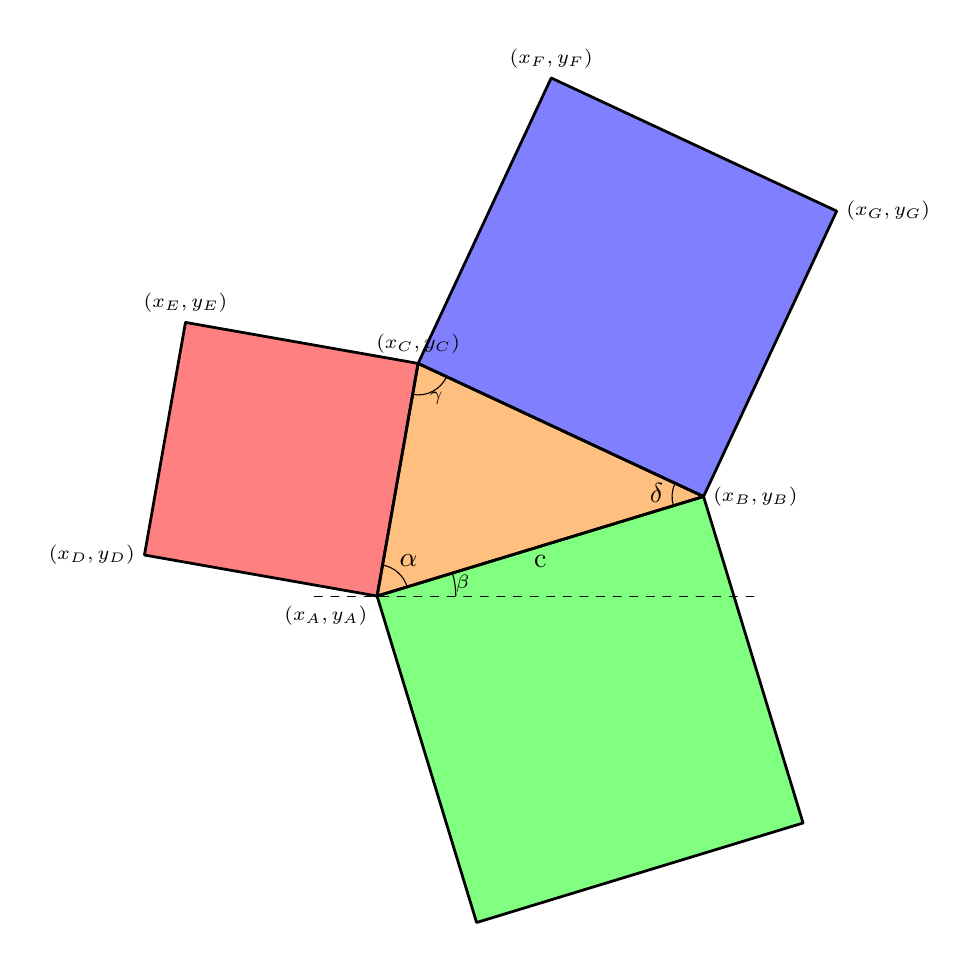
\begin{tikzpicture}[background rectangle/.style={fill=white!45}, show background rectangle]
  \tkzInit
  % Defining the triangle
  \tkzDefPoint(0,0){C}
  \begin{scope}[shift=(C)]
    \tkzDefPoint(-100:3){A}
    \tkzDefPoint(-25:4){B}
  \end{scope}
  \tkzDefShiftPoint[A](4,0){O}
  \tkzDefSquare(B,A)\tkzGetPoints{H}{I}
  \tkzDefSquare(A,C)\tkzGetPoints{E}{D}
  \tkzDefSquare(C,B)\tkzGetPoints{G}{F}
  \tkzFillPolygon[fill = red!50 ](A,C,E,D)
  \tkzFillPolygon[fill = blue!50 ](C,B,G,F)
  \tkzFillPolygon[fill = green!50](B,A,H,I)
  \tkzFillPolygon[fill = orange,opacity=.5](A,B,C)
  \tkzDrawPolygon[line width = 1pt](A,B,C)
  \tkzDrawPolygon[line width = 1pt](A,C,E,D)
  \tkzDrawPolygon[line width = 1pt](C,B,G,F)
  \tkzDrawPolygon[line width = 1pt](B,A,H,I)
  % Labels
  % Points
  \tkzLabelPoint[below left](A){\scriptsize $(x_A, y_A)$}
  \tkzLabelPoint[right](B){\scriptsize $(x_B, y_B)$}
  \tkzLabelPoint[above](C){\scriptsize $(x_C, y_C)$}
  \tkzLabelPoint[left](D){\scriptsize $(x_D, y_D)$}
  \tkzLabelPoint[above](E){\scriptsize $(x_E, y_E)$}
  \tkzLabelPoint[above](F){\scriptsize $(x_F, y_F)$}
  \tkzLabelPoint[right](G){\scriptsize $(x_G, y_G)$}
  % Segments
  \tkzLabelSegment[below](A,B){c}
  % Horizontal line through A
  \tkzDefLine(A,O)
  \tkzDrawLine[dashed](A,O)
  % Marking angles
  \tkzMarkAngle[size=.4](A,C,B)
  \tkzLabelAngle[pos=.5](A,C,B){\scriptsize $\gamma$}
  % Angle BAC
  \tkzMarkAngle[size=.4](B,A,C)
  \tkzLabelAngle[pos=.6](B,A,C){$\alpha$}
  % Angle ABC
  \tkzMarkAngle[size=.4](C,B,A)
  \tkzLabelAngle[pos=.6](C,B,A){$\delta$}
  % Phase of AC
  \tkzMarkAngle[size=1](O,A,B)
  \tkzLabelAngle[pos=1.1](O,A,B){\scriptsize $\beta$}

\end{tikzpicture}
\end{document}


%%% Local Variables:
%%% mode: latex
%%% TeX-master: "figure2"
%%% End:
